%%%%%%%%%%%%%%%%%%%%%%%%%%%%%%%%%%%%%%%%%%%%%%%%%%%%%%%%%%%%%%%%%%%%%%%%%%%%
% AGUJournalTemplate.tex: this template file is for articles formatted with LaTeX
%
% This file includes commands and instructions
% given in the order necessary to produce a final output that will
% satisfy AGU requirements, including customized APA reference formatting.
%
% You may copy this file and give it your
% article name, and enter your text.
% guidelines and troubleshooting are here: 

%% To submit your paper:
%% NOTES:
% DON'T USE SUBFIGURES!!!!



\documentclass[draft]{AR_analysis_}
% \usepackage{hyperref} % creates a hyperlink to the figure referenced
\usepackage{url} %this package should fix any errors with URLs in refs.
\usepackage{lineno}
%for better track changes. finalnew option will compile document with changes incorporated.
\usepackage[inline]{trackchanges}
\usepackage{soul}
\usepackage{float}  % Required for the [H] option
\usepackage{graphicx} % for my graphics
\usepackage{xcolor} % for my graphics
\usepackage{textcomp} % removes warning in gensymb
\usepackage{gensymb} % for basic symbols like degree
\usepackage{mathtools}
\usepackage{amsmath}
\usepackage{tabularx}
%\usepackage{subcaption}

\usepackage{makecell}
\usepackage{array}

\newcolumntype{R}[1]{>{\raggedleft\arraybackslash}m{#1}}

% Bottom four packages from matplotlib -> LaTeX 
% Tutorial
% https://blog.timodenk.com/exporting-matplotlib-plots-to-latex/
\usepackage{tikz}
\usepackage{tikz-cd}
\usepackage{pgfplots}
\pgfplotsset{compat=1.14}

\linenumbers

%%%%%%%
% As of 2018 we recommend use of the TrackChanges package to mark revisions.
% The trackchanges package adds five new LaTeX commands:
%
%  \note[editor]{The note}
%  \annote[editor]{Text to annotate}{The note}
%  \add[editor]{Text to add}
%  \remove[editor]{Text to remove}
%  \change[editor]{Text to remove}{Text to add}
%
% complete documentation is here: http://trackchanges.sourceforge.net/
%%%%%%%

\draftfalse

%% Enter journal name below.
%% Choose from this list of Journals:
%
% JGR: Atmospheres
% JGR: Biogeosciences
% JGR: Earth Surface
% JGR: Oceans
% JGR: Planets
% JGR: Solid Earth
% JGR: Space Physics
% Global Biogeochemical Cycles
% Geophysical Research Letters
% Paleoceanography and Paleoclimatology
% Radio Science
% Reviews of Geophysics
% Tectonics
% Space Weather
% Water Resources Research
% Geochemistry, Geophysics, Geosystems
% Journal of Advances in Modeling Earth Systems (JAMES)
% Earth's Future
% Earth and Space Science
% Geohealth
%
% ie, \journalname{Water Resources Research}

\journalname{Geophysical Research Letters}

\begin{document}

%%%%%%%%%%%%%%%%%%%%%%%%%%%%%%%%%%%%%%%%%%%%%%%
%  TITLE
%
% (A title should be specific, informative, and brief. Use
% abbreviations only if they are defined in the abstract. Titles that
% start with general keywords then specific terms are optimized in
% searches)
%
%%%%%%%%%%%%%%%%%%%%%%%%%%%%%%%%%%%%%%%%%%%%%%%

\title{Influence of Atmospheric Rivers on Alaskan River Ice}

%%%%%%%%%%%%%%%%%%%%%%%%%%%%%%%%%%%%%%%%%%%%%%%
%
%  AUTHORS AND AFFILIATIONS
%
%%%%%%%%%%%%%%%%%%%%%%%%%%%%%%%%%%%%%%%%%%%%%%%

% Authors are individuals who have significantly contributed to the
% research and preparation of the article. Group authors are allowed, if
% each author in the group is separately identified in an appendix.)

% List authors by first name or initial followed by last name and
% separated by commas. Use \affil{} to number affiliations, and
% \thanks{} for author notes.
% Additional author notes should be indicated with \thanks{} (for
% example, for current addresses).

\authors{Russ Limber\affil{1, 2}, Elias Massoud\affil{2}, 
Jitendra Kumar\affil{2}, Forrest M. Hoffman\affil{2}}
\affiliation{1}{The University of Tennessee}
\affiliation{2}{Oak Ridge National Laboratory}

% \affiliation{3}{Third Affiliation}
% \affiliation{4}{Fourth Affiliation}

%(repeat as many times as is necessary)

% Corresponding author mailing address and e-mail address:

% (include name and email addresses of the corresponding author.  More
% than one corresponding author is allowed in this LaTeX file and for
% publication; but only one corresponding author is allowed in our
% editorial system.)

% Example: \correspondingauthor{First and Last Name}{email@address.edu}
\correspondingauthor{Russ Limber}{r62@ornl.gov}


%%%%%%%%%%%%%%%%%%%%%%%%%%%%%%%%%%%%%%%%%%%%%%%
% KEY POINTS
%%%%%%%%%%%%%%%%%%%%%%%%%%%%%%%%%%%%%%%%%%%%%%%
%  List up to three key points (at least one is required)
%  Key Points summarize the main points and conclusions of the article
%  Each must be 140 characters or fewer with no special characters 
% or punctuation and must be complete sentences

% Example:
% \begin{keypoints}
% \item	List up to three key points (at least one is required)
% \item	Key Points summarize the main points and conclusions of the article
% \item	Each must be 140 characters or fewer with no special 
	% characters or punctuation and must be complete sentences
% \end{keypoints}

% These are all under 140 characters
\begin{keypoints}
\item Atmospheric Rivers (ARs) correlate to a one week increase in daily temperature

\item Robust ARs occuring during the coldest period of the year appear to 
	prolong the annual breakup
	date of river ice

\item ARs account for about one third (36\%) of total precipitation and 
	explain almost half (48\%)
 	of interannual variability of precipitation
\end{keypoints}

%%%%%%%%%%%%%%%%%%%%%%%%%%%%%%%%%%%%%%%%%%%%%%%
%
%  ABSTRACT and PLAIN LANGUAGE SUMMARY
%
% A good Abstract will begin with a short description of the problem
% being addressed, briefly describe the new data or analyses, then
% briefly states the main conclusion(s) and how they are supported and
% uncertainties.

% The Plain Language Summary should be written for a broad audience,
% including journalists and the science-interested public, that will not have 
% a background in your field.
%
% A Plain Language Summary is required in GRL, JGR: Planets, JGR: Biogeosciences,
% JGR: Oceans, G-Cubed, Reviews of Geophysics, and JAMES.
% see http://sharingscience.agu.org/creating-plain-language-summary/)
%
%%%%%%%%%%%%%%%%%%%%%%%%%%%%%%%%%%%%%%%%%%%%%%%

%% \begin{abstract} starts the second page
%% The Abstract should be a single paragraph of fewer than 250 words
%% (for Geophysical Research Letters, under 150 words). 

\begin{abstract}

	Atmospheric rivers (ARs) transport vast amounts of moisture from
	low latitudes, mainly the Tropics, to high latitude regions. 
	One region particularly impacted
	by ARs is Alaska USA. We analyze the role of ARs in raising local temperatures, 
	their effect on precipitation variability, and their influence on the annual river
	ice breakup date for 25 locations. Precipitation and 
	temperature records were provided by Daymet, with ARs determined from the Guan and 
	Waliser tracking algorithm. We found ARs increase local temperatures for as long as 
	one week post landfall, account for 36\% of total precipitation and explain 48\% 
	of precipitation variability. Calculating the heat transport between ARs and river 
	ice, fused with a temporal bias, we conclude that heavy precipitation events 
	(HPEs) during the coldest period of the year prolong river ice breakup dates, 
	while HPEs occurring close to the breakup date have little impact on breakup timing. 

\end{abstract}

% The PLS should be a single paragraph no more than 200 words long.
\section*{Plain language summary}

	We strategically selected 25 locations with annual river ice
	breakup dates recorded throughout Interior Alaska. Across all
	locations, we determined that daily temperature increases by up to
	one week post an atmospheric river (AR). We also found that ARs
	account for 36\% of total annual precipitation from 1980 to 2023
	and explain 48\% of the variability of precipitation. We then
	calculated the total heat transfer between precipitation and river
	ice while taking into account a bias function for time.
	Surprisingly, we found that heavy precipitation events (HPEs),
	both local precipitation and ARs, that occur relatively close to
	river ice breakup dates, have little correlation to the breakup
	date. However, HPEs that occur during the coldest period of the
	year (typically late December to mid-January) are strongly inversely
	correlated with river ice breakup timing, and therefore prolong
	the breakup date.

%%%%%%%%%%%%%%%%%%%%%%%%%%%%%%%%%%%%%%%%%%%%%%%
%
%  BODY TEXT
%
%%%%%%%%%%%%%%%%%%%%%%%%%%%%%%%%%%%%%%%%%%%%%%%

%%% Suggested section heads:
% \section{Introduction}
%
% The main text should start with an introduction. Except for short
% manuscripts (such as comments and replies), the text should be divided
% into sections, each with its own heading.

% Headings should be sentence fragments and do not begin with a
% lowercase letter or number. Examples of good headings are:

% \section{Materials and Methods}
% Here is text on Materials and Methods.
%
% \subsection{A descriptive heading about methods}
% More about Methods.
%
% \section{Data} (Or section title might be a descriptive heading about data)
%
% \section{Results} (Or section title might be a descriptive heading about the
% results)
%
% \section{Conclusions}



\section{Introduction}

Atmospheric rivers (ARs) are narrow corridors of intense water vapor
transport that significantly influence hydrologic events, transporting
most of the water vapor outside of the Tropics \cite{NOAA_AR_summary}.
It is estimated that ARs are responsible for as much as 90\% of poleward
water vapor transport at midlatitudes \cite{other_alg}. ARs contribute to
extreme precipitation events across various regions worldwide, including
Western North America \cite{Dettinger2004, Neiman2008, Guan2010,
ARs_flood_WA_State, ARs_flood_Russian_River_CA, Ralph2013, ARs_CA}
Europe \cite{Lavers2013, ARs_impact_Norway}, and Western South America
\cite{ARs_impact_SA}. In recent years, the impacts of ARs on the
cryosphere have been more extensively analyzed. It was found that between
1981 and 2020 atmospheric moisture content anticorrelates significantly
with sea ice concentration over almost the entire Arctic Ocean
\cite{ARs_lead_to_sea_ice_loss}. For those same years, another analysis
found that 100\% of extreme temperature events in the Arctic (above 0
$\degree C$) coincides with ARs \cite{Ma2023}. Many analyses have noted
a relationship between heavy AR activity and sea ice loss, caused by
increased rainfall from moisture originating in lower latitudes
\cite{Zhang2023, maclennan_contribution_2022}. However Arctic systems
are complicated, as the intense moisture transport within ARs can also
result in heavy snowfall events, thus contributing to the accumulation
of snowpack, especially in mountainous regions \cite{Saavedra2020,
Guan2010}. Under the right conditions, this relationship has been found
to actually increase the mass balance of glaciers \cite{Little2019}.
Understanding the role of ARs in the cryosphere is essential for
assessing their broader impact on regional water resources and glacier
dynamics in a changing climate. While a number of works have explored
the relationship between ARs and sea ice, to our knowledge there haven't
been any analyses that look at the relationship between ARs and Arctic
river ice. Many works have used physics based processes and allometrics
to model the annual breakup timing and conditions of Arctic river ice
\cite{Paily, ashton1986river, Prowse_Bonsal_Duguay_Lacroix_2007,
jasek1998, shen_newest}. While it is recognized that an increase in
streamflow alters the dynamics surrounding river ice breakup timing
\cite{ashton1986river}, the relationship precipitation, and to that end
AR timing, has on Arctic river ice has yet to be examined. This analysis
sets out to answer the following questions: 1.) Is there a change in
air temperature for each location corresponding to the timing of ARs?
2.) How do ARs contribute to precipitation throughout interior Alaska?
3.) Do ARs impact the timing of river ice breakup?

\section{Data}

Similar to previous studies, we define ARs using integrated vapor
transport (IVT) values constructed from 6-hourly values of 3‐D wind and
water vapor at eight pressure levels between 300 and 1,000
mb from the NCEP/NCAR reanalysis data product \cite{NCEP_NCAR_reanalysis}. 
AR detection is based on version3 of the tARget algorithm
\cite{Guan_Waliser2019, bin2022}.
The IVT values are calculated at the original
resolution from the National Center for Environmental Protection (NCEP)
meteorological inputs \cite{NCEP_reanalysis}. AR frequency for a given
period within each grid cell is calculated by taking the number of days
that detect an AR and dividing by the total number of days in that
period. Therefore, for a given grid cell, AR frequency of 0\% means
there were no AR conditions at any of the time steps and frequency of
100\% means there were AR conditions at every time step. Guan and
Waliser \cite{alg_for_detecting_AR_moisture_fluxes} developed a global
AR detection algorithm, which was updated and validated later with in
situ and dropsonde data \cite{bin2022}. This algorithm is employed for
our study, which is based on a combination of the IVT magnitude,
direction, and geometry characteristics, to objectively identify ARs.
Contiguous regions of enhanced IVT transport are first identified from
magnitude thresholding (i.e., grid cells with IVT above the seasonally
and regionally dependent $85^{th}$ percentile) and further filtered
using directional and geometry criteria requirements. The detection
algorithm was applied to NCEP in its native resolution of $2.5 \degree$.
This detection algorithm had over 90\% agreement in detected AR
landfall dates with other methods for detecting ARs made for Western
North America \cite{Neiman2008}, the United Kingdom \cite{Lavers2011}, 
and East Antarctica \cite{Gorodetskaya2014}. Precipitation and daily
minimum and maximum temperatures ($T_{\text{min}}$ and $T_{\text{max}}$) 
were imported from Oak Ridge National
Laboratory's Daymet $1kmx1km$ daily product, via the
Distributed Active Archive Center \cite{daymet}. River ice breakup dates 
were collected from the Alaska Pacific River Forecast Center database 
(APRFC). While exact coordinates were unavailable, coordinates were 
approximated based on proximity to weather stations and airports to 
maintain spatial consistency with inputs used in Daymet’s meteorological 
models. 25 locations were identified as having at least 35 breakup 
records between 1980 and 2023 (the current temporal availability of 
Daymet). 35 was used as the threshold because it allowed for the greatest 
number of locations with the most complete time series 
necessary for statistical analysis.

\begin{figure}
\centering
\includegraphics[width=1.0\textwidth]{./images/concatenated_maps_precip_temp_plot.png}
	\caption{Top: (left) map showing summated precipitation for the
	year 2021; (right) map of average temperature for 2021. Bottom:
	One of the 25 locations (Crooked Creek on the Kuskokwim
	River) for the year 2021. Yellow, orange, red represents the
	temperature profiles (fill plot of $T_{\text{min}}$ -
	$T_{\text{max}}$) from NCEP
	temperature data at 850, 925 and 1000mb respectively. Light
	green represents Daymet temperature profile. Dark blue shows
	modeled precipitation from Daymet while the light blue stem
	plots depict AR events. The purple dashed line shows the breakup
	date for the Kuskokwim River in 2021 for Crooked Creek.}
\label{fig:concatenated_maps_precip_temp_plot} 
\end{figure}

Daymet precipitation, $T_{\text{min}}$ and $T_{\text{max}}$ were used in our analysis as they
have a strong agreement with NCEP temperature outputs for our region of interest
Figure \ref{fig:concatenated_maps_precip_temp_plot}. Additionally, 
because Daymet is derived directly from in-situ instruments 
and meteorological stations, it represents a robust 
standard for precipitation and temperature predictions across North
America \cite{daymet2021}.

\section{Methods}

To determine the impact that ARs have on local temperature, we used a
varying temporal window combined with a pairwise t-test. For each
AR occurence, a lookback window and forecast window each equal to n
days in length was created before and after the AR date, respectively,
whereby: $ n \in \{1, 2, 3, \ldots, 14\}$.
For values of n greater than one day the mean was taken within each window
for $T_{\text{min}}$ and $T_{\text{max}}$. These aggregated temperatures were then
calculated over all locations. Aggregated temperature pairs 
were assessed using a one tailed pairwise t-test to test
whether ARs increase local temperature over period of time n $(\alpha =
0.05)$. We explored how ARs compare to local precipitation events by
separating out precipitation caused by an AR and precipitation not
caused by an AR. We then used the Wilcoxon rank-sum test to test the hypothesis 
that AR events tend to produce more precipitation than local
precipitation events (the distributions of precipitation were shown to
not be normally distributed even after log transformation using the
Shapiro-Wilks test hence the use of a non-parametric test). We calculate
the interannual variability of precipitation that ARs account for by
conducting a univariate ordinary least squares regression (OLS). To
determine the impact that ARs have on river ice breakup timing heat
transport was estimated using Equation \ref{eq:heat_transport}:

\begin{equation}
\frac{dQ}{dt} = \alpha \cdot m \cdot \Delta T 
	\label{eq:heat_transport}
\end{equation}

\noindent where $Q$ is heat flux ($\frac{J}{m^2}$); $\alpha$ specific heat 
($\frac{J}{g \cdot \degree C}$); $\Delta T$ is the difference of 
ambient temperature and the river ice surface (which is estimated 
using $T_{\text{min}}$ as a proxy for ambient) ($\degree C$); $m$ 
the mass of the precipitation ($kg$). The integral of these values
over all precipitation events that occured seven months prior to the
breakup date is taken with respect to time. A temporal bias function
(Equation \ref{eq:cases})
with tunable parameters is applied to the heat equation to assess when in
time precipitation events were more impactful on breakup timing:

\begin{equation}
	\label{eq:cases}
	f(t; \gamma, \kappa, DOY, c) =
	\begin{cases}
    	\frac{e^{-\gamma \cdot (-t - DOY)} - 1}{\kappa} & \text{if }
        	t < c \\
    	\frac{e^{-\gamma \cdot (t - DOY)} - 1}{\kappa} & \text{if }
        	t \geq c \\
	\end{cases}
\end{equation}

\noindent where $\gamma$ is a tunable parameter impacting the width of
the exponential function; t is time; DOY is the day of year
that the breakup date occured; c is a tunable parameter dictating the
center placement of the function $\kappa$ is a normalizing constant.
Finally, Equation \ref{eq:final_eq} is tuned using a full grid search, for each
location optimized by the Pearson correlation coefficient. 

\begin{equation}
\label{eq:final_eq}
	\int_{t_i}^{t_{DOY}} \left(f(t; \gamma, \kappa, DOY, c) \cdot
	\frac{dQ}{dt}\right) \, dt
\end{equation}



\section{Results} 

The pairwise t-test comparing n length lookback and forecast windows
found that based on an $\alpha = 0.05$ there is a
statistically significant difference in $T_{\text{min}}$ n days prior to an AR event
to n days after, when $ n \in \{1, \ldots, 10\}$ on average.
This was true for all locations in the study when $ n \in \{1,
\ldots, 8\}$, at which point the p-values become insignificant for some
locations. The t-test for
tmax implies that the presence of an AR has less of an effect, with
statistical significance found when $ n \in \{1, \ldots, 6\}$ on
average. Some locations showed no significance when $n=1$ and $n=6$. Figure
\ref{fig:tmin_vs_tmax_subplots} shows the change in p-values for each
value of n (top row) as well as the mean increase in temperature
from the lookback window to the forecast window. The mean
temperatures are higher for $T_{\text{min}}$ post AR than tmax, with both plots
showing a clear downward trend as the length of n increases.     

\begin{figure}
\centering
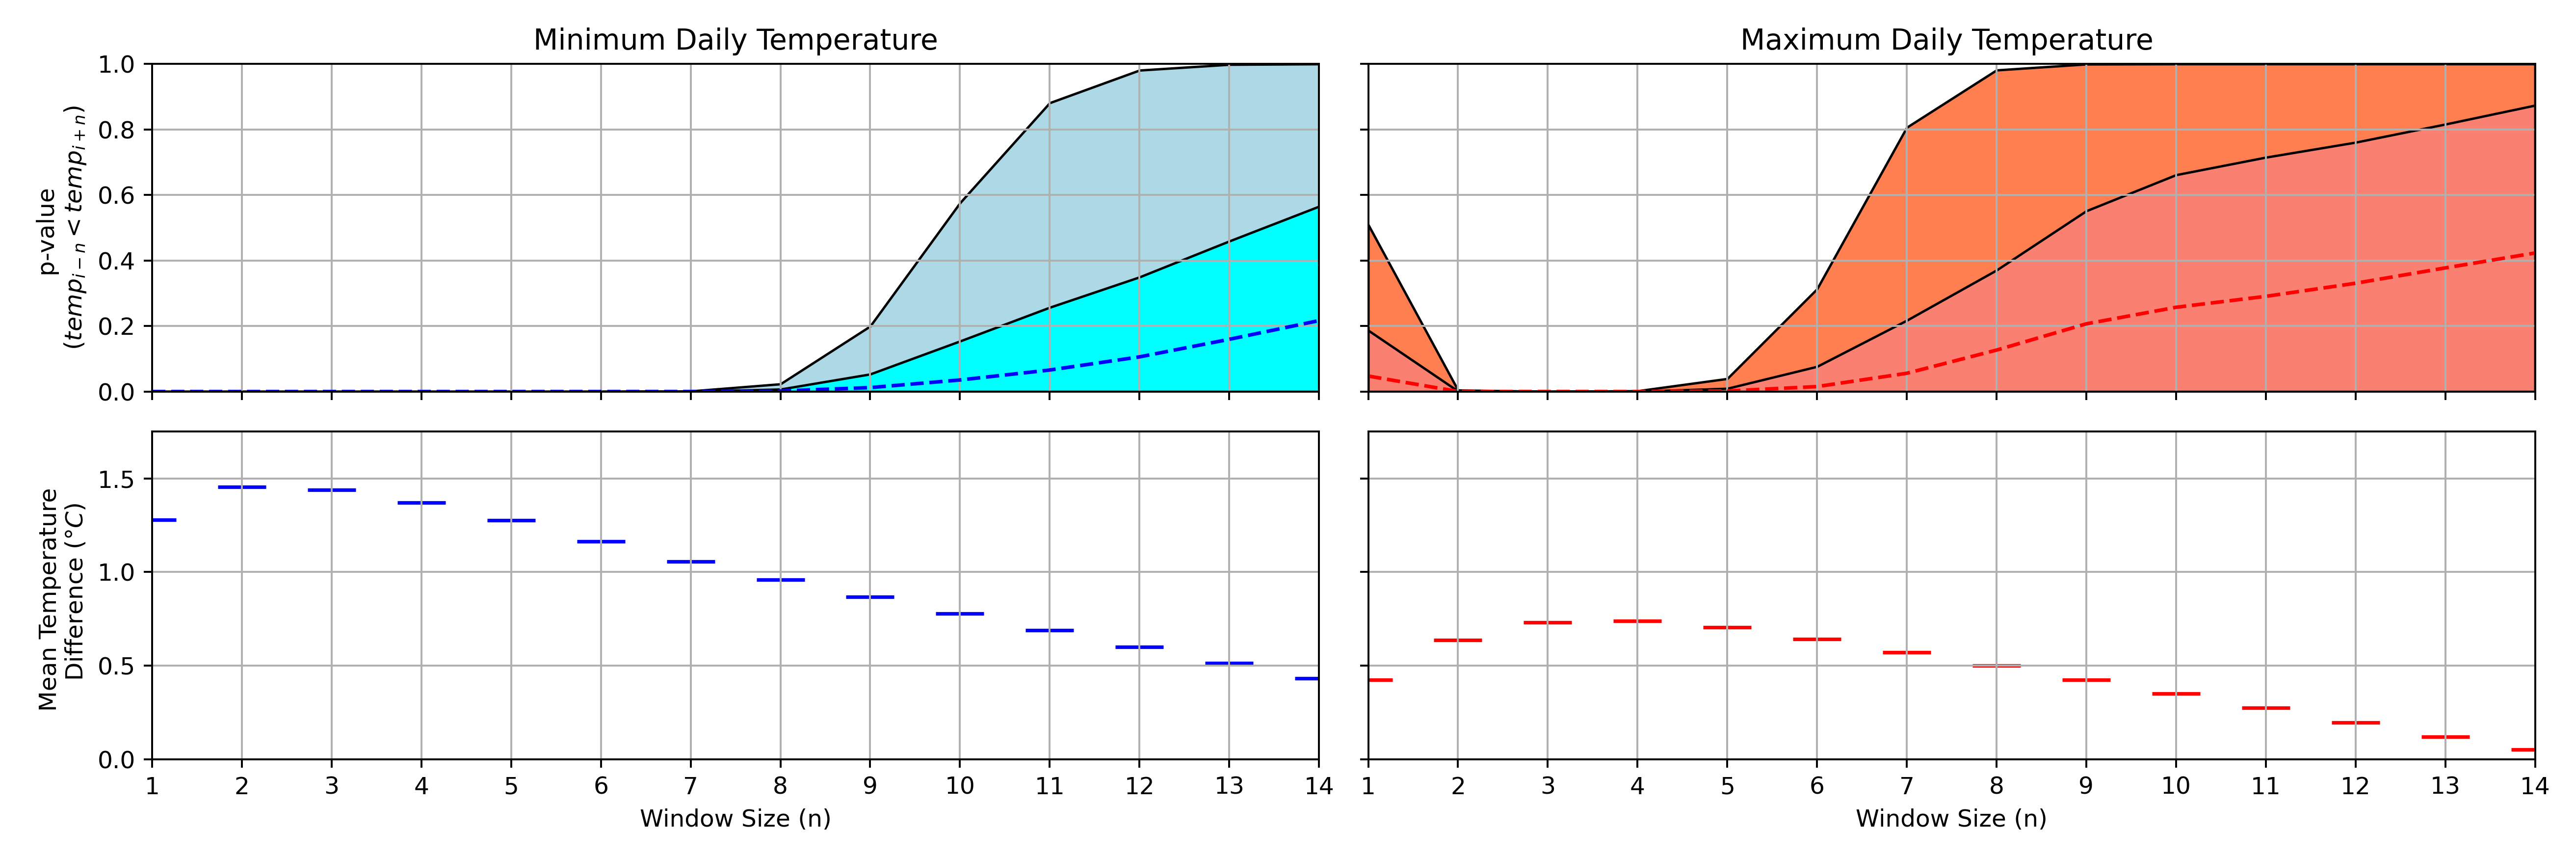
\includegraphics[width=1.0\textwidth]{./images/tmin_vs_tmax_subplots.png}
\caption{Top: the p-value of the paired t-test given the
	window size surrounding the AR event date. Dashed lines
	represent the mean p-value over the study area while the color
	transition depicts the IQR of p-values Bottom: the average increase
	in temperature from the lookback window to the forecast window.}
\label{fig:tmin_vs_tmax_subplots} 
\end{figure}

Figure \ref{fig:IVT_Precip_proportion_over_time} shows the temporal
trends in aggregated IVT and precipitation,
over all locations. Interannually, ARs tend to account for 36\% of
precipitation on average, with a high degree of variability given
the year and location (Figure \ref{fig:IVT_Precip_proportion_over_time}
bottom row). The results from the Wilcoxin rank-sum test show that
precipitation from ARs tends to be greater than non-AR precipitation
($\text{test statistic} = -83.85; \text{ p-value} \approx 0.0)$. It
was found that of the top 5\% of all precipitation events, 57\% were
caused by ARs (Figure \ref{fig:concatenated_precip_var_plots} left).
Using annual aggregated precipitation from ARs to model total annual
aggregated precipitation in a univariate OLS we find that the
coefficient of variation ($R^{2}$) is equal to 0.48. This means that ARs
explain about 48\% of interannaul variability in precipitation.  

\begin{figure}
\centering
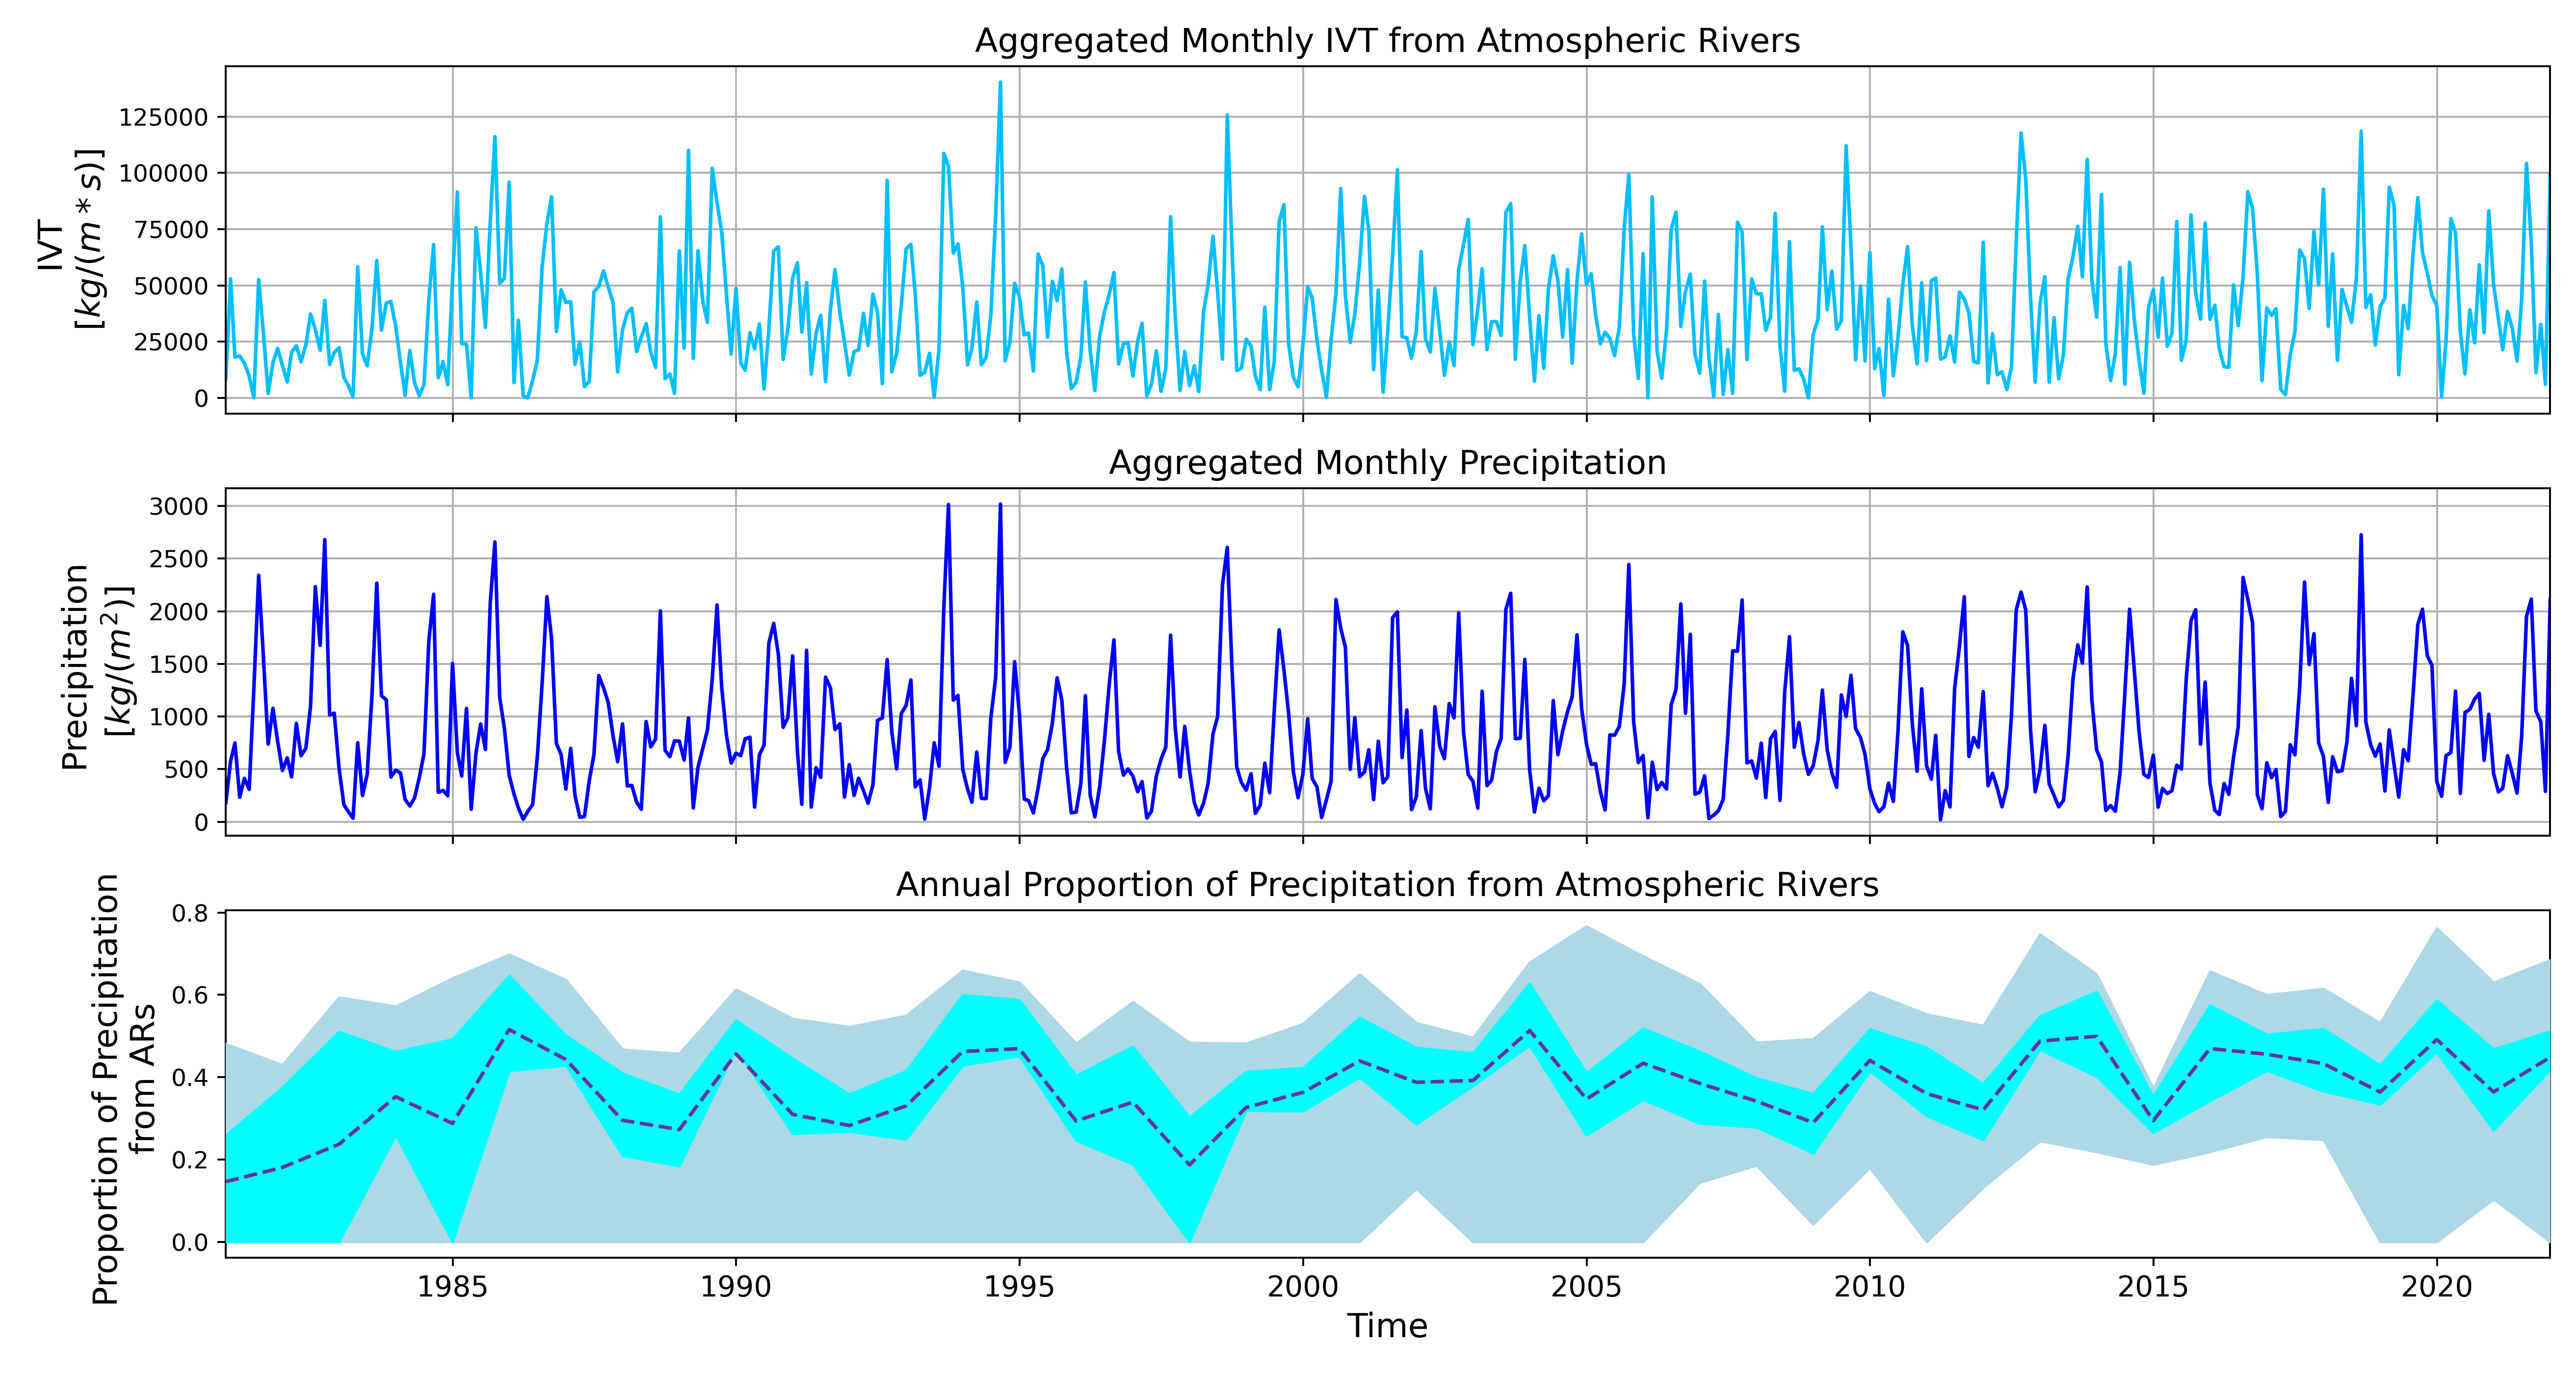
\includegraphics[width=1.0\textwidth]{./images/IVT_Precip_proportion_over_time.png}
\caption{Top: time series of IVT aggregated over all locations.
	Middle: time series of precipitation aggregated monthly over all
	locations. Bottom: proportion of precipitation accounted for by
	ARs, fill colors depict IQR while dashed line depicts the mean,
	aggregated over all locations annually. }
\label{fig:IVT_Precip_proportion_over_time}
\end{figure}

Lastly, using Equation \ref{eq:final_eq} to calculate the heat transfer
between precipitation and the river ice surface, we note that there is a
strong negative correlation between the heat transfer and DOY (Figure
\ref{fig:concatenated_precip_var_plots} upper left) when the bias curve
is positioned during the coldest period of the year - typically near
January 1st \ref{fig:concatenated_precip_var_plots} upper right). In
this context, negative values along the y-axis of the left column 
of the scatterplots are interpretted
as a negative heat exchange, meaning a cooling effect on the river ice
surface or a deposition of precipitation below freezing. Equation
\ref{eq:final_eq} was optimized through adjusting the tunable parameters
within the temporal bias (Equation \ref{eq:cases}) on a location by
location basis. For example, Crooked Creek on the Kuskokwim River has a
clear negative trend with more robust, colder HPE causing a cooling effect on the
river ice surface, prolonging DOY, with a Pearson correlation
coefficient $ (r_{p} )= -0.84$ and a Spearman correlation coefficient
$(r_{s}) = -0.80$ . The relationship between the total
number of ARs that occured six months prior to the breakup date and the
DOY are shown in the center column (top and bottom plots are the same by
definition) indicating that the number of ARs prior to river ice breakup
appears insufficient in correlating to breakup timing on its own. The
bottom row of Figure \ref{fig:concatenated_corr_plots} shows that the
use of a bias function is necessary, as simply applying the integral of
Equation \ref{eq:heat_transport} (the aggregated total heat transfer) is
poorly uncorrelated. 


\begin{figure}
\centering
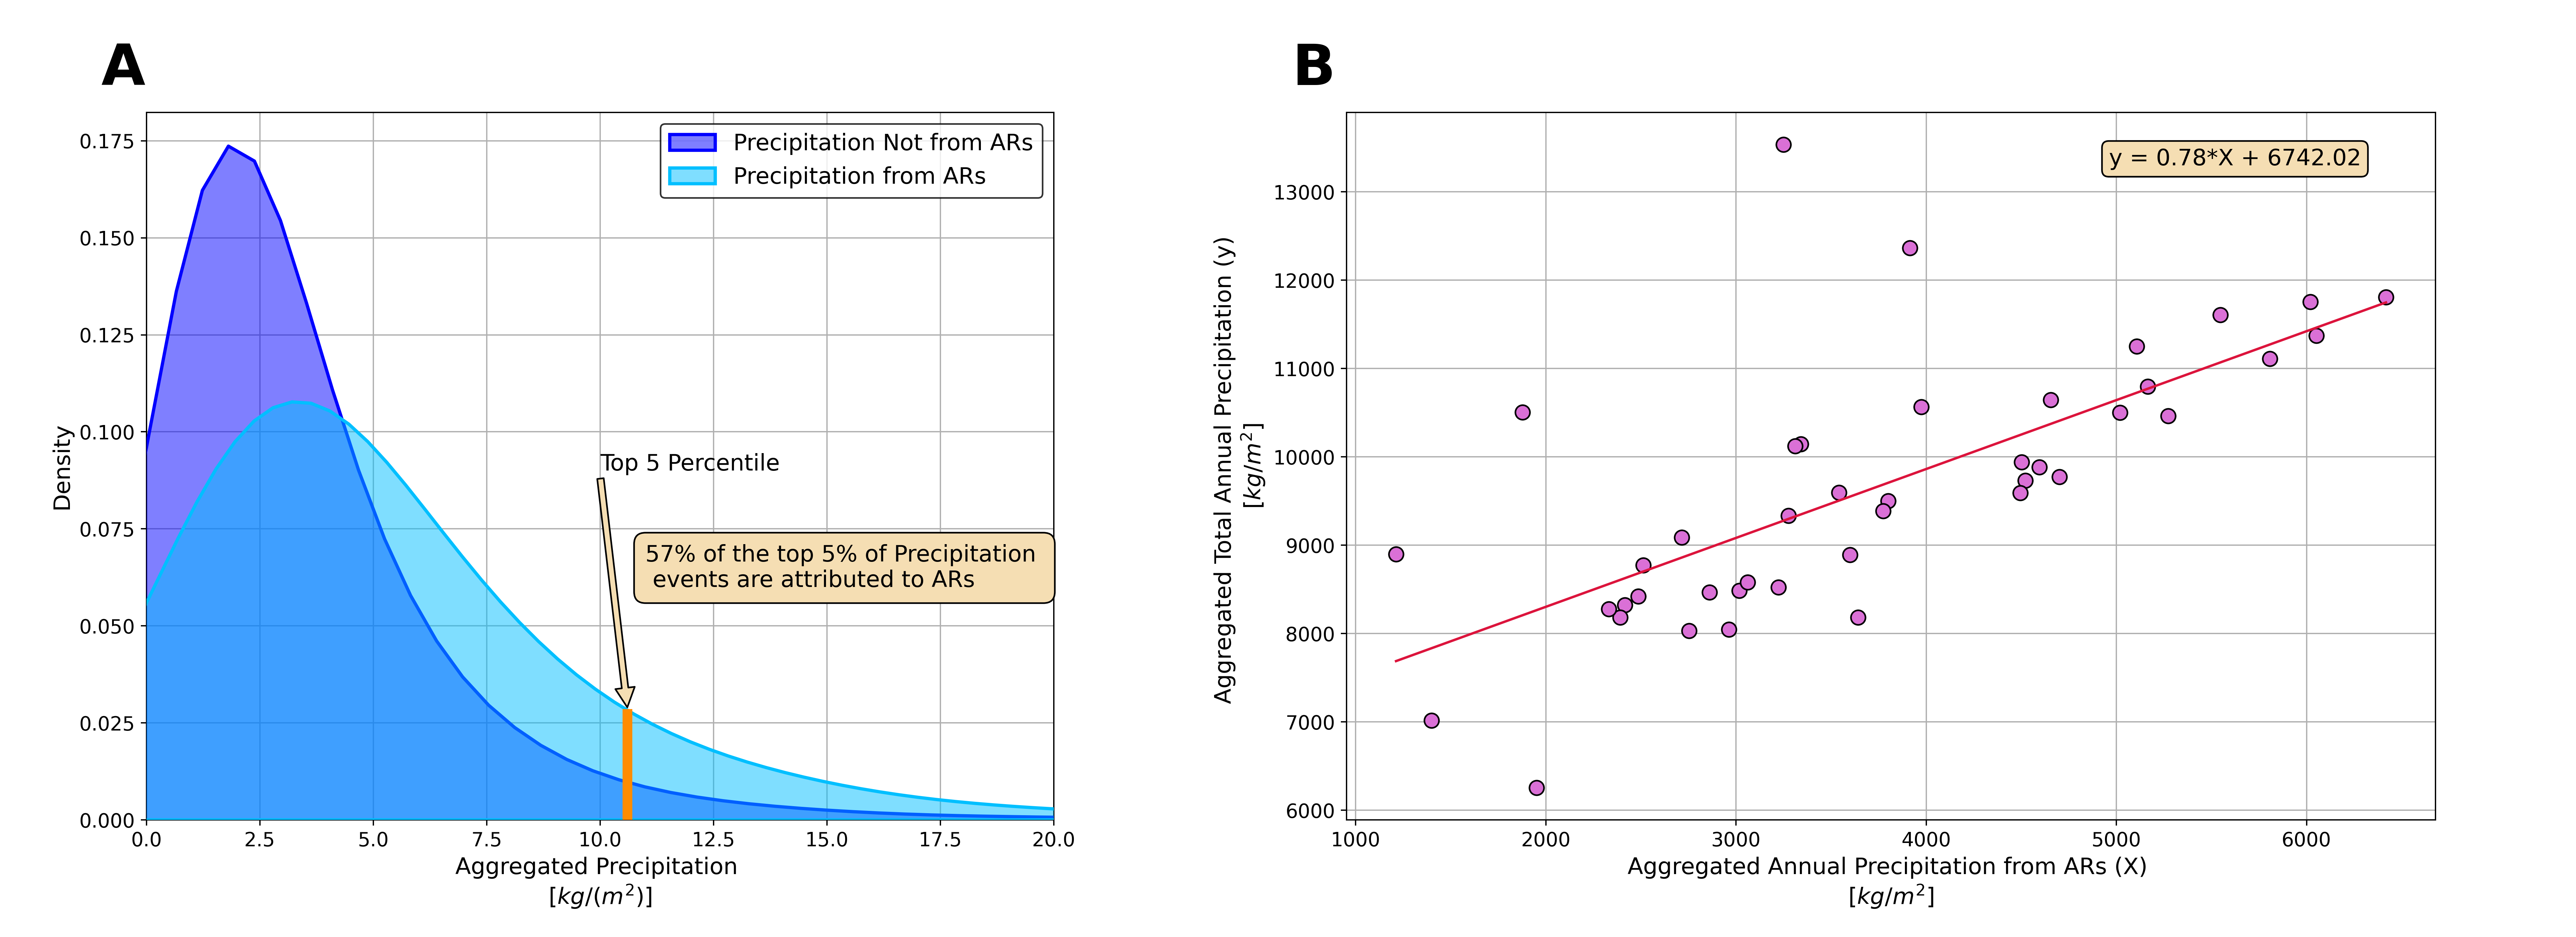
\includegraphics[width=1.0\textwidth]{./images/concatenated_precip_var_plots.png}
\caption{Left: kernel density plots showing the distribution of
	local precipitation (dark blue) and precipitation from ARs
	(light blue). Right: orindary least squares regression plot
	using annual, summated precipitation from ARs, to predict annual
	summated precipitation.}
\label{fig:concatenated_precip_var_plots}
\end{figure}

\begin{figure}
\centering
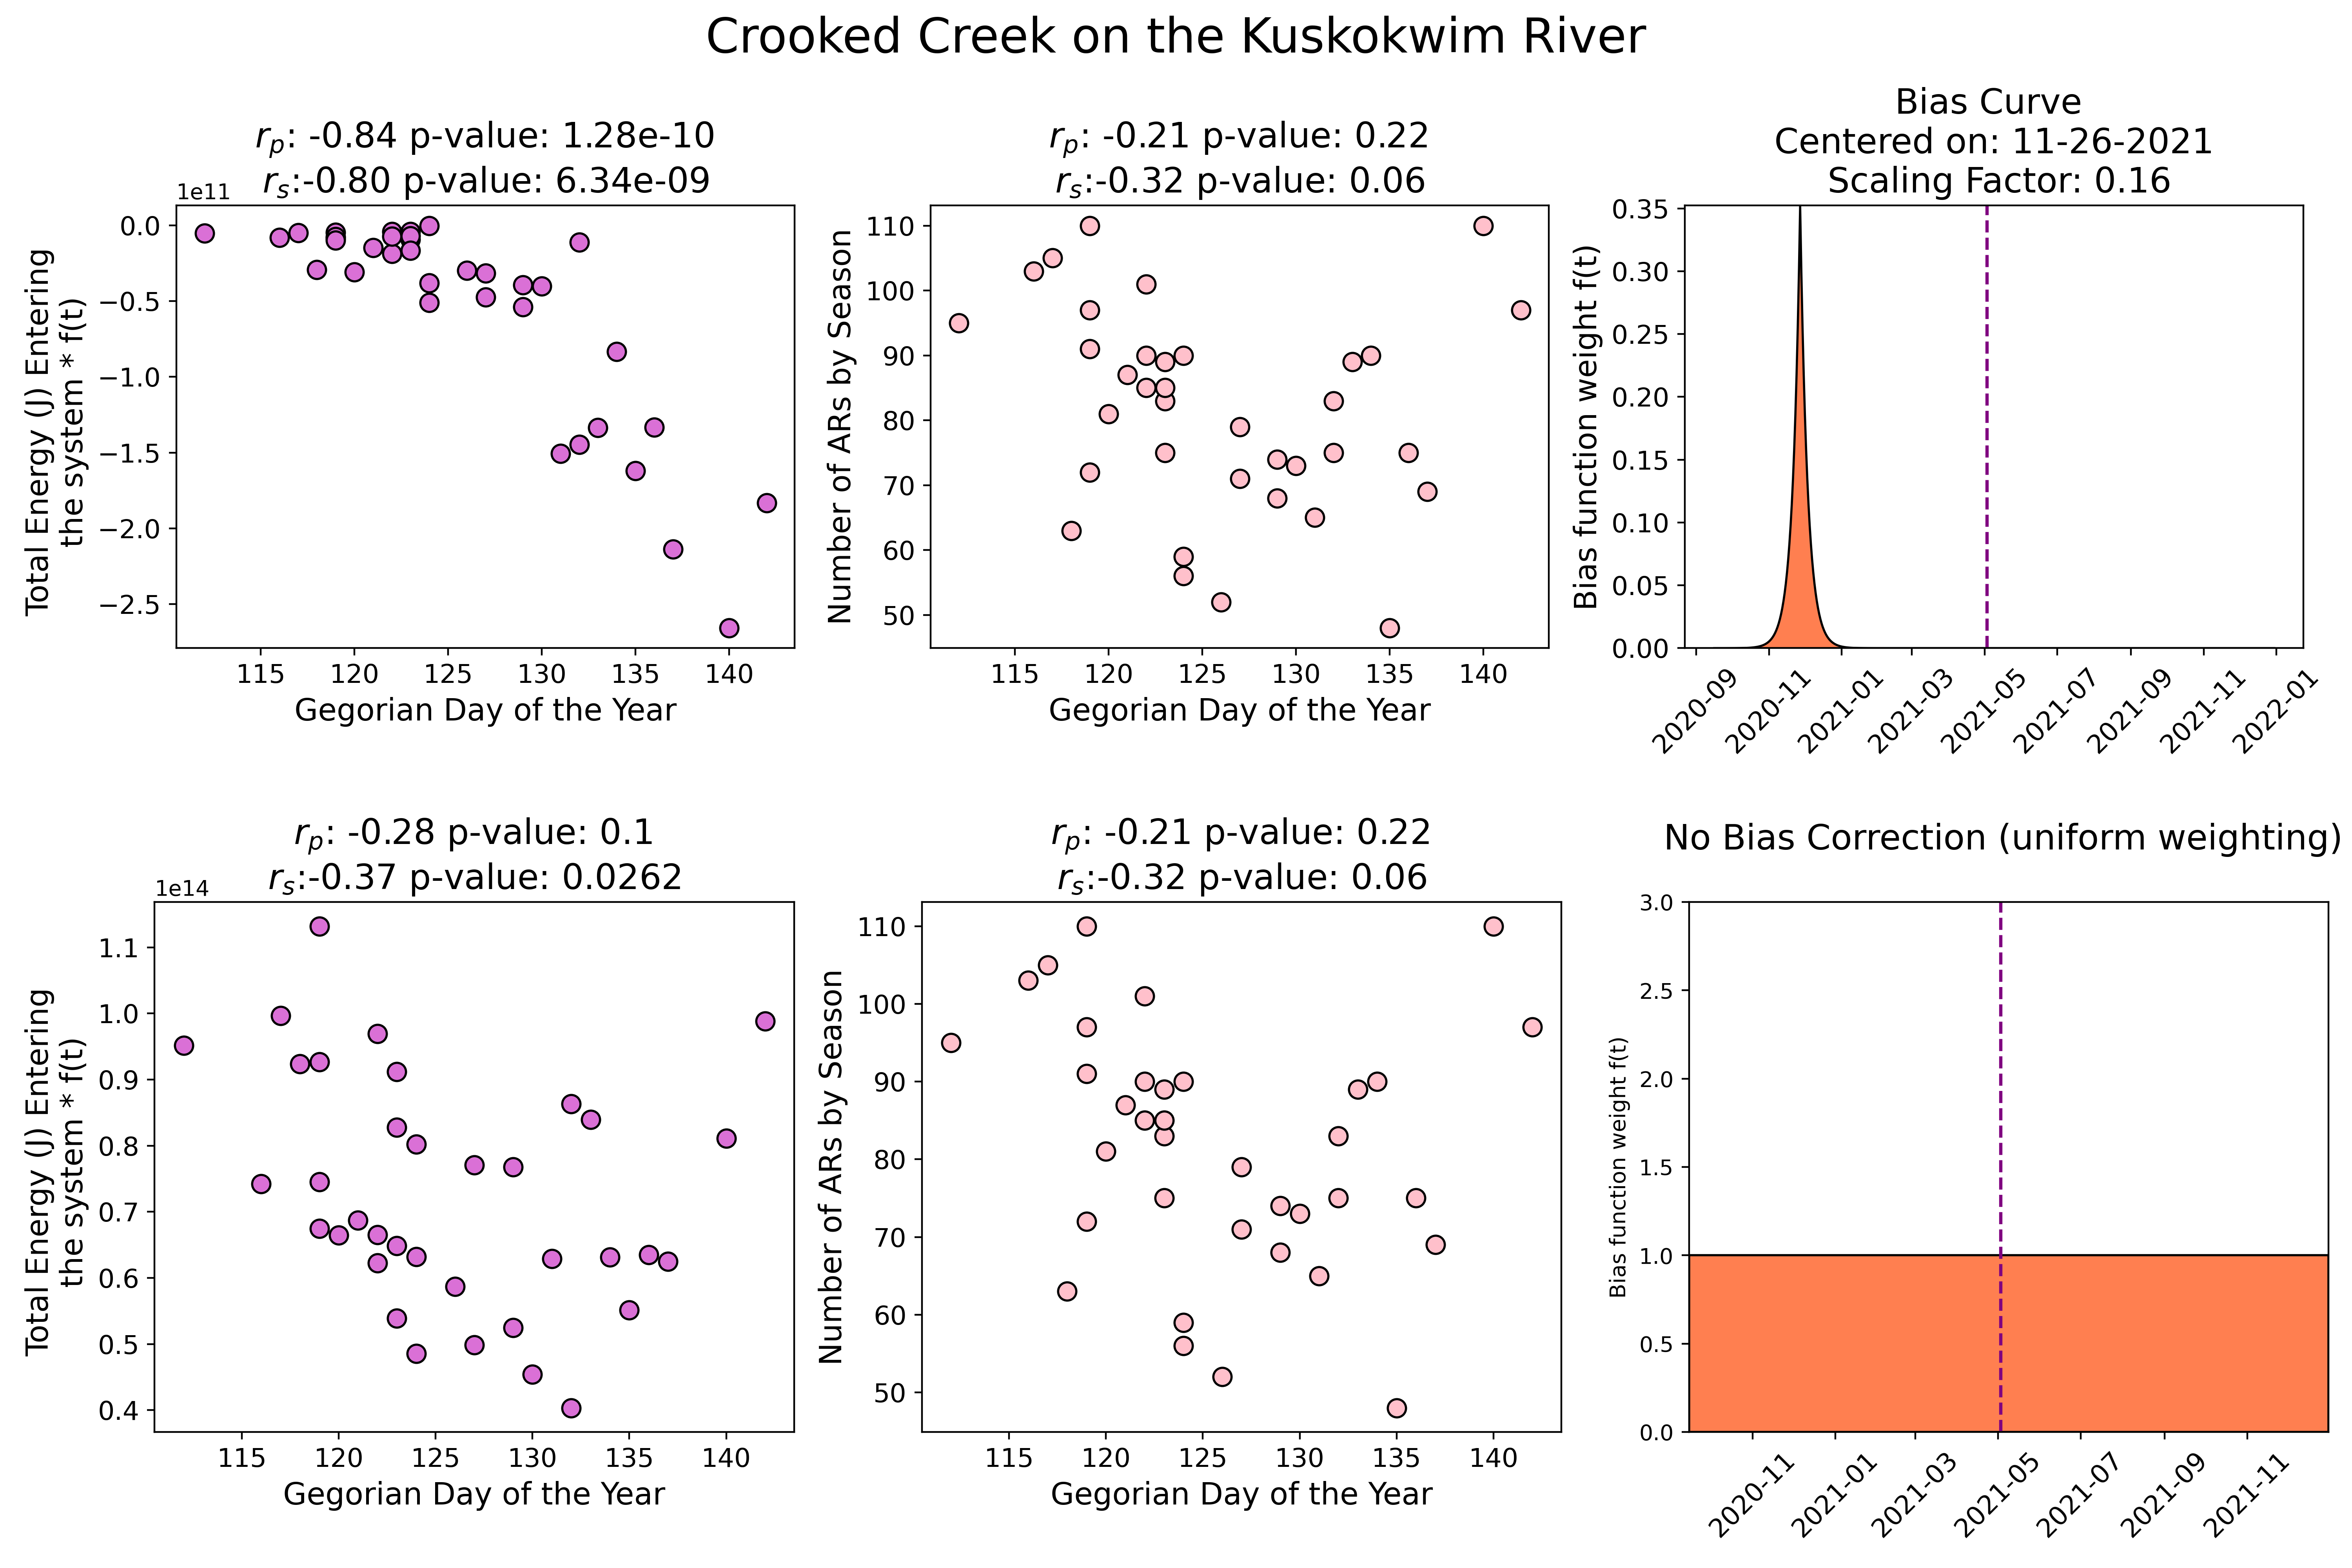
\includegraphics[width=1.0\textwidth]{./images/concatenated_scatter_bias_plots.png}
	\caption{Top: (left) scatter plot between thermal energy
	transfer and DOY; (middle) scatter plot of the number of ARs
	that occured in the six months prior to the breakup date and
	DOY; 
	(right) temporal bias curve for the year 2021 with the breakup
	date represented by the vertical dashed line. Bottom: same as
	the top except depicting the results when a temporal bias
	is not utilized.}
\label{fig:concatenated_corr_plots}
\end{figure}

\section{Conclusion and Discussion}


%%%%%%%%%%%%%%%%%%%%%%%%%%%%%%%%%%%%%%%%%%%%%%%
%
% DATA SECTION and ACKNOWLEDGMENTS
%
%%%%%%%%%%%%%%%%%%%%%%%%%%%%%%%%%%%%%%%%%%%%%%%

\section*{Open research section}
This section MUST contain a statement that describes where the data supporting the conclusions
can be obtained. Data cannot be listed as ''Available from authors'' or stored solely in 
supporting information. Citations to archived data should be included in your reference
list. Wiley will publish it as a separate section on the paper’s page. Examples and 
complete information are here:
https://www.agu.org/Publish with AGU/Publish/Author Resources/Data for Authors


\acknowledgments
Enter acknowledgments here. This section is to acknowledge funding, thank colleagues, 
enter any secondary affiliations, and so on.


%%%%%%%%%%%%%%%%%%%%%%%%%%%%%%%%%%%%%%%%%%%%%%%
% REFERENCES and BIBLIOGRAPHY
%
% \bibliography{<name of your .bib file>} don't specify the file extension
% don't specify bibliographystyle
%
%%%%%%%%%%%%%%%%%%%%%%%%%%%%%%%%%%%%%%%%%%%%%%%

%\bibliography{ enter your bibtex bibliography filename here }
\bibliography{AR_analysis_}


%Reference citation instructions and examples:
%
% Please use ONLY \cite and \citeA for reference citations.
% \cite for parenthetical references
% ...as shown in recent studies (Simpson et al., 2019)
% \citeA for in-text citations
% ...Simpson et al. (2019) have shown...
%
%
%...as shown by \citeA{jskilby}.
%...as shown by \citeA{lewin76}, \citeA{carson86}, \citeA{bartoldy02}, and \citeA{rinaldi03}.
%...has been shown \cite{jskilbye}.
%...has been shown \cite{lewin76,carson86,bartoldy02,rinaldi03}.
%... \cite <i.e.>[]{lewin76,carson86,bartoldy02,rinaldi03}.
%...has been shown by \cite <e.g.,>[and others]{lewin76}.
%
% apacite uses < > for prenotes and [ ] for postnotes
% DO NOT use other cite commands (e.g., \citet, \citep, \citeyear, \nocite, \citealp, etc.).
%

\appendix
\section*{Appendix A.}


\end{document}






































% More Information and Advice:

%%

%  Numbered lines in equations:
%  To add line numbers to lines in equations,
%  \begin{linenomath*}
%  \begin{equation}
%  \end{equation}
%  \end{linenomath*}



%% Enter Figures and Tables near as possible to where they are first mentioned:
%
% DO NOT USE \psfrag or \subfigure commands.
%
% Figure captions go below the figure.
% Acronyms used in figure captions will be spelled out in the final, published version.

% Table titles go above tables;  other caption information
%  should be placed in last line of the table, using
% \multicolumn2l{$^a$ This is a table note.}
% NOTE that there is no difference between table caption and table heading in the final, published version
%
%----------------
% EXAMPLE FIGURES
%
% \begin{figure}
% \includegraphics{example.png}
% \caption{caption}
% \end{figure}
%
% Giving latex a width will help it to scale the figure properly. A simple trick is to use 
% \textwidth. Try this if large figures run off the side of the page.
% \begin{figure}
% \noindent\includegraphics[width=\textwidth]{anothersample.png}
%\caption{caption}
%\label{pngfiguresample}
%\end{figure}
%
%
% If you get an error about an unknown bounding box, try specifying the width and height 
% of the figure with the natwidth and natheight options. This is common when trying to add a PDF figure without pdflatex.
% \begin{figure}
% \noindent\includegraphics[natwidth=800px,natheight=600px]{samplefigure.pdf}
%\caption{caption}
%\label{pdffiguresample}
%\end{figure}
%
%
% PDFLatex does not seem to be able to process EPS figures. You may want to try the epstopdf package.
%

%
% ---------------
% EXAMPLE TABLE
%
% \begin{table}
% \caption{Time of the Transition Between Phase 1 and Phase 2$^{a}$}
% \centering
% \begin{tabular}{l c}
% \hline
%  Run  & Time (min)  \\
% \hline
%   $l1$  & 260   \\
%   $l2$  & 300   \\
%   $l3$  & 340   \\
%   $h1$  & 270   \\
%   $h2$  & 250   \\
%   $h3$  & 380   \\
%   $r1$  & 370   \\
%   $r2$  & 390   \\
% \hline
% \multicolumn{2}{l}{$^{a}$Footnote text here.}
% \end{tabular}
% \end{table}

%%%%%%%%%%%%%%%%%%%%%%%%%%%%%%%%%%%%%%%%%%%%%%%
% SIDEWAYS FIGURES and TABLES
% AGU prefers the use of {sidewaystable} over {landscapetable} as it causes fewer problems.
%
% \begin{sidewaysfigure}
% \includegraphics[width=20pc]{figsamp}
% \caption{caption here}
% \label{newfig}
% \end{sidewaysfigure}
%
%  \begin{sidewaystable}
%  \caption{Caption here}
% \label{tab:signif_gap_clos}
%  \begin{tabular}{ccc}
% one&two&three\\
% four&five&six
%  \end{tabular}
%  \end{sidewaystable}

%% If using numbered lines, please surround equations with \begin{linenomath*}...\end{linenomath*}
%\begin{linenomath*}
%\begin{equation}
%y|{f} \sim g(m, \sigma),
%\end{equation}
%\end{linenomath*}

%%% End of body of article

%%%%%%%%%%%%%%%%%%%%%%%%%%%%%%%%%%%%%%%%%%%%%%%
%% Optional Appendices go here
%
% The \appendix command resets counters and redefines section heads
%
% After typing \appendix
%
%\section{Here Is Appendix Title}
% will show
% A: Here Is Appendix Title
%

%%%%%%%%%%%%%%%%%%%%%%%%%%%%%%%%%%%%%%%%%%%%%%%
% Optional Glossary, Notation or Acronym section goes here:
%
% Glossary is only allowed in Reviews of Geophysics
%  \begin{glossary}
%  \term{Term}
%   Term Definition here
%  \term{Term}
%   Term Definition here
%  \term{Term}
%   Term Definition here
%  \end{glossary}


%%%%%%%%%%%%%%%%%%%%%%%%%%%%%%%%%%%%%%%%%%%%%%%
% Acronyms
%% NOTE that acronyms in the final published version will be spelled out when used in figure captions.
%   \begin{acronyms}
%   \acro{Acronym}
%   Definition here
%   \acro{EMOS}
%   Ensemble model output statistics
%   \acro{ECMWF}
%   Centre for Medium-Range Weather Forecasts
%   \end{acronyms}


%%%%%%%%%%%%%%%%%%%%%%%%%%%%%%%%%%%%%%%%%%%%%%%
% Notation
%   \begin{notation}
%   \notation{$a+b$} Notation Definition here
%   \notation{$e=mc^2$}
%   Equation in German-born physicist Albert Einstein's theory of special
%  relativity that showed that the increased relativistic mass ($m$) of a
%  body comes from the energy of motion of the body—that is, its kinetic
%  energy ($E$)—divided by the speed of light squared ($c^2$).
%   \end{notation}


%%%%%%%%%%%%%%%%%%%%%%%%%%%%%%%%%%%%%%%%%%%%%%%
%
%  SECTION HEADS
%
%%%%%%%%%%%%%%%%%%%%%%%%%%%%%%%%%%%%%%%%%%%%%%%

% Capitalize the first letter of each word (except for
% prepositions, conjunctions, and articles that are
% three or fewer letters).

% AGU follows standard outline style; therefore, there cannot be a section 1 without
% a section 2, or a section 2.3.1 without a section 2.3.2.
% Please make sure your section numbers are balanced.
% ---------------
% Level 1 head
%
% Use the \section{} command to identify level 1 heads;
% type the appropriate head wording between the curly
% brackets, as shown below.
%
%An example:
%\section{Level 1 Head: Introduction}
%
% ---------------
% Level 2 head
%
% Use the \subsection{} command to identify level 2 heads.
%An example:
%\subsection{Level 2 Head}
%
% ---------------
% Level 3 head
%
% Use the \subsubsection{} command to identify level 3 heads
%An example:
%\subsubsection{Level 3 Head}
%
%---------------
% Level 4 head
%
% Use the \subsubsubsection{} command to identify level 3 heads
% An example:
%\subsubsubsection{Level 4 Head} An example.
%
%%%%%%%%%%%%%%%%%%%%%%%%%%%%%%%%%%%%%%%%%%%%%%%
%
%  IN-TEXT LISTS
%
%%%%%%%%%%%%%%%%%%%%%%%%%%%%%%%%%%%%%%%%%%%%%%%
%
% Do not use bulleted lists; enumerated lists are okay.
% \begin{enumerate}
% \item
% \item
% \item
% \end{enumerate}
%
%%%%%%%%%%%%%%%%%%%%%%%%%%%%%%%%%%%%%%%%%%%%%%%
%
%  EQUATIONS
%
%%%%%%%%%%%%%%%%%%%%%%%%%%%%%%%%%%%%%%%%%%%%%%%

% Single-line equations are centered.
% Equation arrays will appear left-aligned.

%Math coded inside display math mode \[ ...\]
% will not be numbered, e.g.,:
% \[ x^2=y^2 + z^2\]

% Math coded inside \begin{equation} and %\end{equation} will
% be automatically numbered, e.g.,:
% \begin{equation}
% x^2=y^2 + z^2
% \end{equation}


% To create multiline equations, use the
% \begin{eqnarray} and \end{eqnarray} environment
% as demonstrated below.
%\begin{eqnarray}
 % x_{1} & = & (x - x_{0}) \cos \Theta \nonumber \\
 %       && + (y - y_{0}) \sin \Theta  \nonumber \\
%  y_{1} & = & -(x - x_{0}) \sin \Theta \nonumber \\
 %       && + (y - y_{0}) \cos \Theta.
%\end{eqnarray}

%If you don't want an equation number, use the star form:
%\begin{eqnarray*}...\end{eqnarray*}

% Break each line at a sign of operation
% (+, -, etc.) if possible, with the sign of operation
% on the new line.

% Indent second and subsequent lines to align with
% the first character following the equal sign on the
% first line.

% Use an \hspace{} command to insert horizontal space
% into your equation if necessary. Place an appropriate
% unit of measure between the curly braces, e.g.
% \hspace{1in}; you may have to experiment to achieve
% the correct amount of space.


%%%%%%%%%%%%%%%%%%%%%%%%%%%%%%%%%%%%%%%%%%%%%%%
%
%  EQUATION NUMBERING: COUNTER
%
%%%%%%%%%%%%%%%%%%%%%%%%%%%%%%%%%%%%%%%%%%%%%%%

% You may change equation numbering by resetting
% the equation counter or by explicitly numbering
% an equation.

% To explicitly number an equation, type \eqnum{}
% (with the desired number between the brackets)
% after the \begin{equation} or \begin{eqnarray}
% command.  The \eqnum{} command will affect only
% the equation it appears with; LaTeX will number
% any equations appearing later in the manuscript
% according to the equation counter.
%

% If you have a multiline equation that needs only
% one equation number, use a \nonumber command in
% front of the double backslashes (\\) as shown in
% the multiline equation above.

% If you are using line numbers, remember to surround
% equations with \begin{linenomath*}...\end{linenomath*}

%  To add line numbers to lines in equations:
%  \begin{linenomath*}
%  \begin{equation}
%  \end{equation}
%  \end{linenomath*}



